\documentclass[11pt,a4paper]{article}
\usepackage[utf8]{inputenc}
\usepackage[T1]{fontenc}
\usepackage[left=25mm,right=25mm,top=25mm,bottom=25mm]{geometry}
\usepackage{graphicx}
\usepackage{caption}
\usepackage{amsmath}
\usepackage{booktabs}
\usepackage{array}
\usepackage[hidelinks]{hyperref}
\captionsetup{font=small}
\hypersetup{pdftitle={Lab 4: Explainability, Compression and MANOLO},
pdfauthor={Jorge Ruiz Gonzalez and Hugo Lopez Sola}}
\hypersetup{pageanchor=false}
\begin{document}

\begin{titlepage}
\begin{center}
{
\includegraphics[width=1\textwidth]{logo.png}\par}
\vspace{0.5 cm}
{\bfseries\LARGE Universidad de Zaragoza \par}
\vspace{0.5 cm}
{\scshape\Large Facultad de Ingenier\'ia\par}
\vspace{0.5 cm}
{\scshape\LARGE Artificial Intelligence - Lab Session 4:
Explainability and Model Compression\par}
\vspace{1.5 cm}
\vfill
{\Large Jorge Ruiz Gonz\'alez (826685) \par}
{\Large Hugo L\'opez Sola (875455) \par}
\vfill
{\Large October 20th, 2026 \par}
\end{center}
\end{titlepage}
\hypersetup{pageanchor=true}
\tableofcontents

\clearpage
\section{Task 1: Baseline CNN}
We used the AugCXR dataset to classify chest X-rays as NORMAL or PNEUMONIA.
There are 7,200 training images, 1,800 validation images and 1,000 test images,
with equal numbers from each class. We used grayscale because colour is not
needed for these images, resized them to $128\times128$, and normalized them
using the training data. Horizontal flips were disabled.

We trained ResNet-18 from scratch for 10 epochs with AdamW, a batch size of 64
and an initial learning rate of $0.0003$. The best validation result was at
epoch 7, with about 95.1\% accuracy. Training accuracy later reached 100\%
without improving validation accuracy, which suggests some overfitting.

Test accuracy was \textbf{97.8\%}. Recall was 97.6\% for NORMAL and 98.0\% for
PNEUMONIA. The confusion matrix below shows 22 mistakes in total. Accuracy is
useful here because the classes are balanced, but checking both classes also
shows whether one is being missed more often.

\begin{table}[ht]
\centering
\small
\caption{Confusion matrix on the test set.}
\begin{tabular}{lrr}
\toprule
True class / predicted class & NORMAL & PNEUMONIA\\
\midrule
NORMAL & 488 & 12\\
PNEUMONIA & 10 & 490\\
\bottomrule
\end{tabular}
\end{table}

\section{Task 2: Explainability}
Grad-CAM usually highlighted broad areas inside the chest, although some
heatmaps also reached the borders or corners. In some wrong predictions, the
attention was near an image boundary or a letter marker. This suggests that
the model sometimes uses irrelevant features. Other mistakes still focused
on the chest, so the heatmaps alone do not explain every error. Some wrong
predictions also had high confidence.

The earlier layer, \texttt{layer2}, gave smaller, scattered hotspots.
\texttt{layer4} gave smoother and broader areas, but less detail: its feature
maps are only $4\times4$ for our input size. Grad-CAM++ gave similar main
hotspots to Grad-CAM, with small differences in their shape and intensity.

\section{Task 3: Compression}
Int8 quantization gave the best balance in our notebook. Accuracy only changed
from 97.8\% to 97.7\%, while the saved model became about four times smaller
(44.8 to 11.3 MB). CPU time for a batch of 32 images fell from about 575 to
378 ms, giving roughly a $1.5\times$ speed-up.

\begin{table}[ht]
\centering
\small
\caption{Test accuracy before and after fine-tuning the pruned models.}
\begin{tabular}{lrrrr}
\toprule
Pruned weights & 30\% & 50\% & 70\% & 90\%\\
\midrule
Test accuracy before fine-tuning & 96.5\% & 85.6\% & 50.0\% & 50.0\%\\
After two fine-tuning epochs & 97.4\% & 97.3\% & 97.3\% & 97.1\%\\
\bottomrule
\end{tabular}
\end{table}

Pruning without fine-tuning broke down at 70\% and 90\%, but two training
epochs recovered most of the accuracy. It did not reduce file size or give a
CPU speed-up because the zero weights were still stored and processed in
dense tensors. For int8 calibration, one batch gave 94.9\% validation accuracy
and ten batches gave 95.1\%. One was already close; we kept ten for our final
int8 model.

\clearpage
\section{Task 4: MANOLO workflow}
\subsection{Results and comparison}
We registered the saved model and a dataset containing 2,000 training images
and 1,000 test images. The workflow ran inference, 50\% magnitude pruning
with two fine-tuning epochs, and then 8-bit quantization with one training
epoch. All three tasks finished successfully.

\begin{table}[ht]
\centering
\small
\caption{Accuracy in the notebook and the MANOLO workflow.}
\begin{tabular}{lrr}
\toprule
Experiment & Notebook accuracy & MANOLO accuracy\\
\midrule
Original model & 97.8\% & 97.8\%\\
50\% pruning + fine-tuning & 97.3\% & 96.8\%\\
Quantization & 97.7\% & 96.6\%\\
\bottomrule
\end{tabular}
\end{table}

The original model gave the same accuracy and per-class recall in both runs.
Pruning kept most of the accuracy. In the notebook we quantized the original
model, whereas MANOLO quantized the already pruned model. Its final accuracy
was 1.2 percentage points below the baseline. MANOLO also used fewer training
images for fine-tuning, so the compression experiments are not identical.

Quantization made the saved model about $3.9\times$ smaller in MANOLO,
similar to the notebook. Pruning alone left its size unchanged.

Grad-CAM was enabled in the workflow, but its heatmap report is missing from
the saved files. We could not visually compare it with the notebook results.

\subsection{Extra measurements}
MANOLO also recorded energy use, estimated CO$_2$ emissions, hardware
utilization, confidence and inference throughput.

\begin{table}[ht]
\centering
\small
\caption{Resource measurements recorded by MANOLO.}
\begin{tabular}{lrrr}
\toprule
Step & Duration (s) & Energy (Wh) & CO$_2$ (g)\\
\midrule
Inference & 10.6 & 0.36 & 0.063\\
Pruning & 12.1 & 0.52 & 0.090\\
Quantization & 11.6 & 0.46 & 0.080\\
\bottomrule
\end{tabular}
\end{table}

These measurements include compression and fine-tuning, so they do not show
the energy saved during future use. Average inference batch latency was
about 4 ms on the MANOLO node. This cannot be directly compared with the
notebook's CPU timing because the hardware and setup differ.

\subsection{What MANOLO adds}
The notebook was useful for trying things and inspecting images. MANOLO
registered the data and models, ran the workflow and stored results in
MLflow. This makes experiments easier to repeat and compare, and helps keep
track of which model was used.

Quantization was the most useful compression method here. Pruning recovered
good accuracy after fine-tuning, but did not make the dense model smaller or
faster. We worked on one dataset and did not carry out the optional task.

\clearpage
\subsection{MLflow screenshots}

\begin{figure}[!ht]
\centering
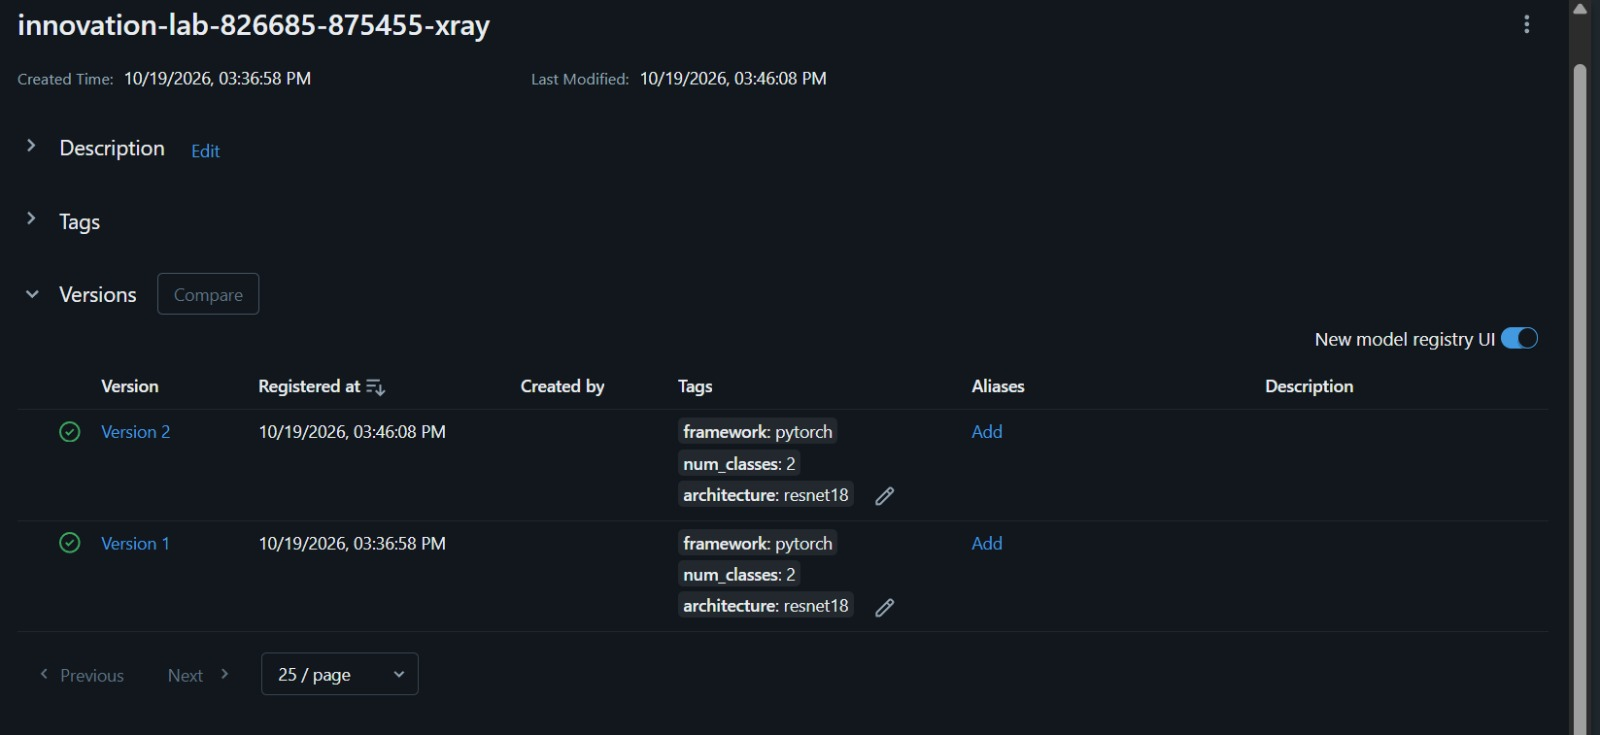
\includegraphics[width=\textwidth,height=0.35\textheight,keepaspectratio]{../manolo/model.jpeg}
\caption{Model registered in MLflow. Version 2 was used in our workflow.}
\end{figure}

\begin{figure}[!ht]
\centering
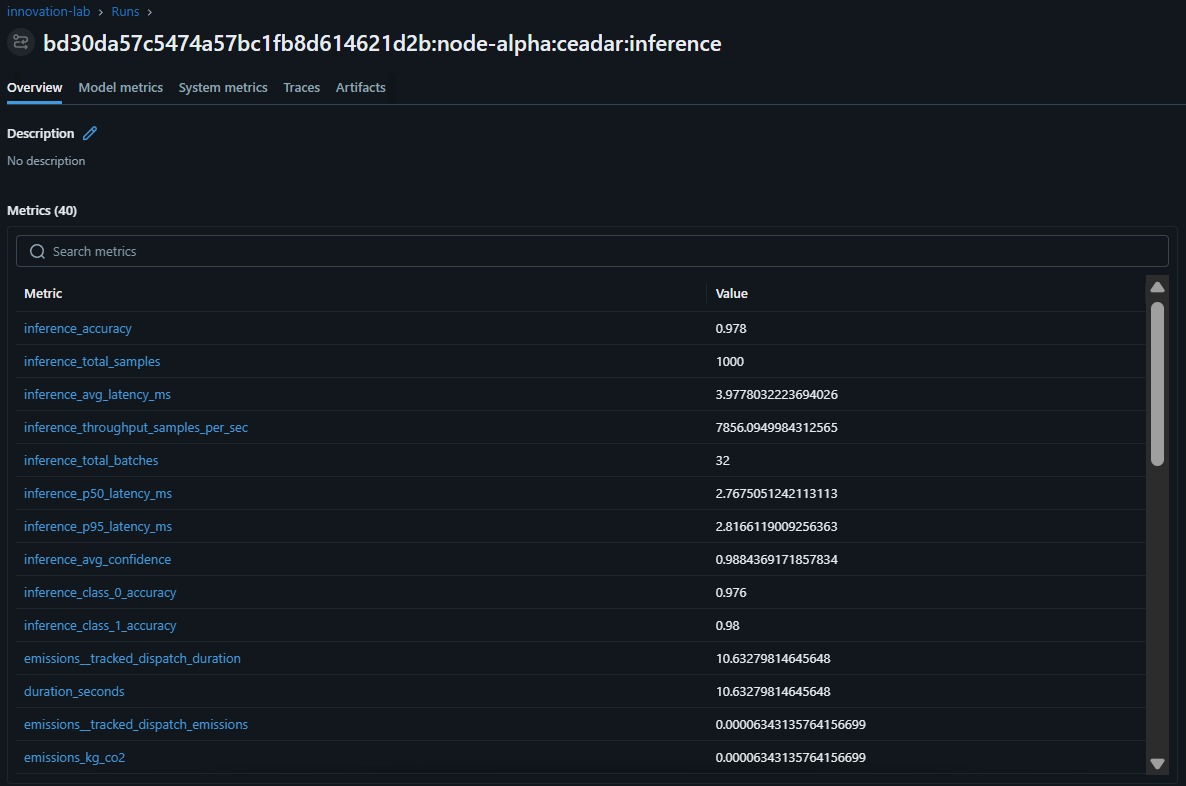
\includegraphics[width=\textwidth,height=0.43\textheight,keepaspectratio]{../manolo/inference.jpeg}
\caption{Inference results: 97.8\% accuracy on the 1,000 test images.}
\end{figure}

\clearpage
\begin{figure}[!ht]
\centering
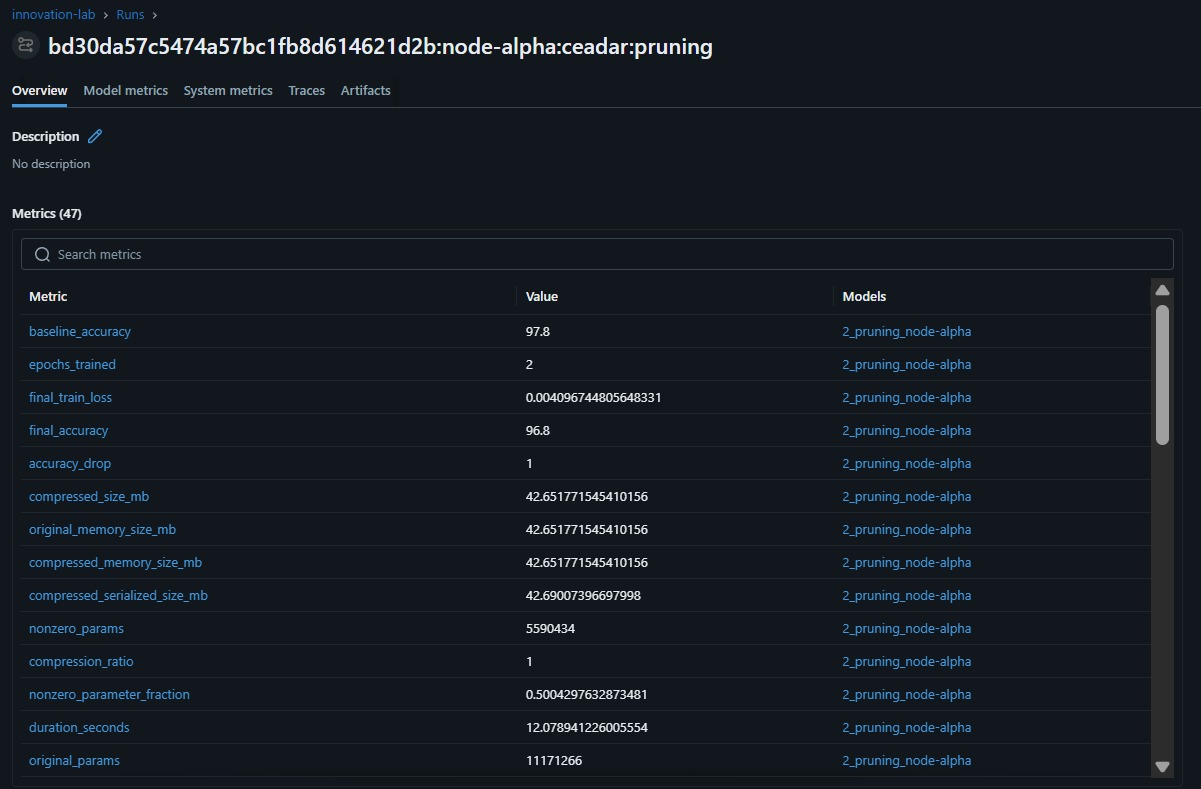
\includegraphics[width=\textwidth,height=0.43\textheight,keepaspectratio]{../manolo/pruning.jpeg}
\caption{Pruning results: 96.8\% accuracy after two fine-tuning epochs.}
\end{figure}

\begin{figure}[!ht]
\centering
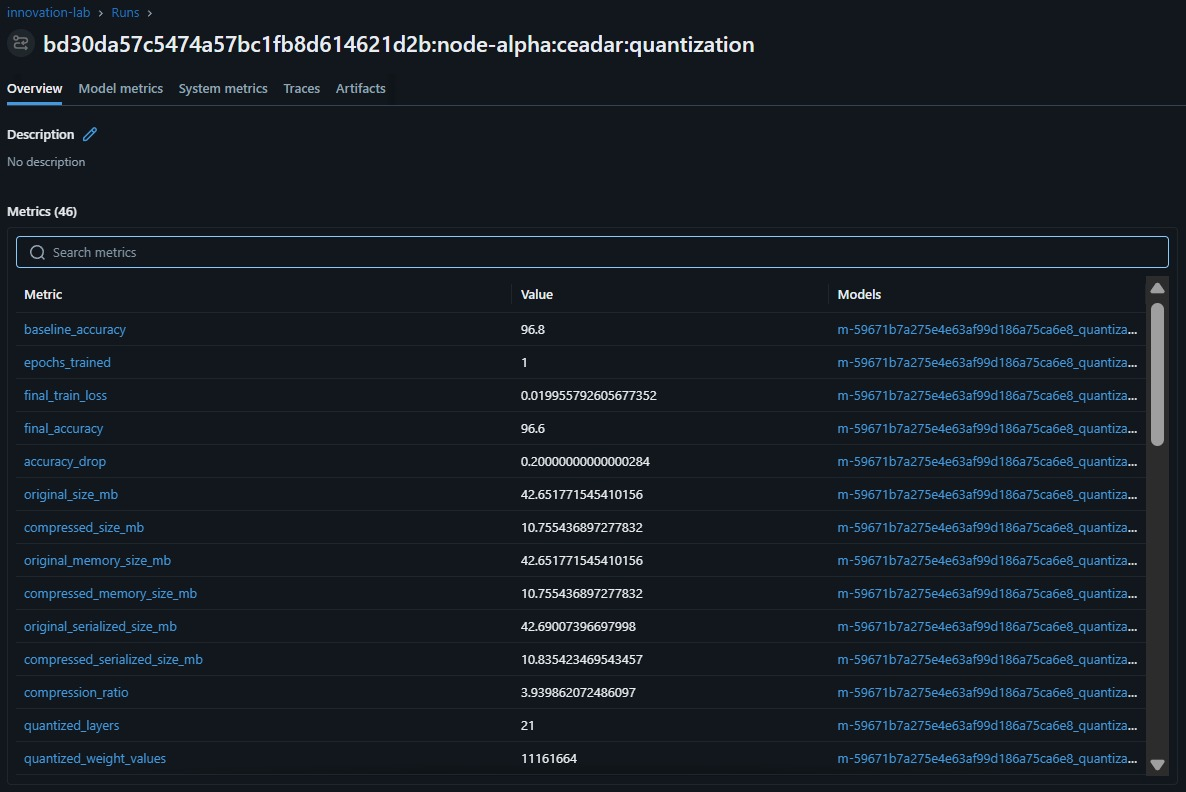
\includegraphics[width=\textwidth,height=0.43\textheight,keepaspectratio]{../manolo/quantization.jpeg}
\caption{Quantization of the pruned model: 96.6\% accuracy and about four times smaller size.}
\end{figure}

\end{document}
